\begin{frame}
\frametitle{Renderizzare Un Colore: Demo}
\begin{figure}[ht]
    \centering
    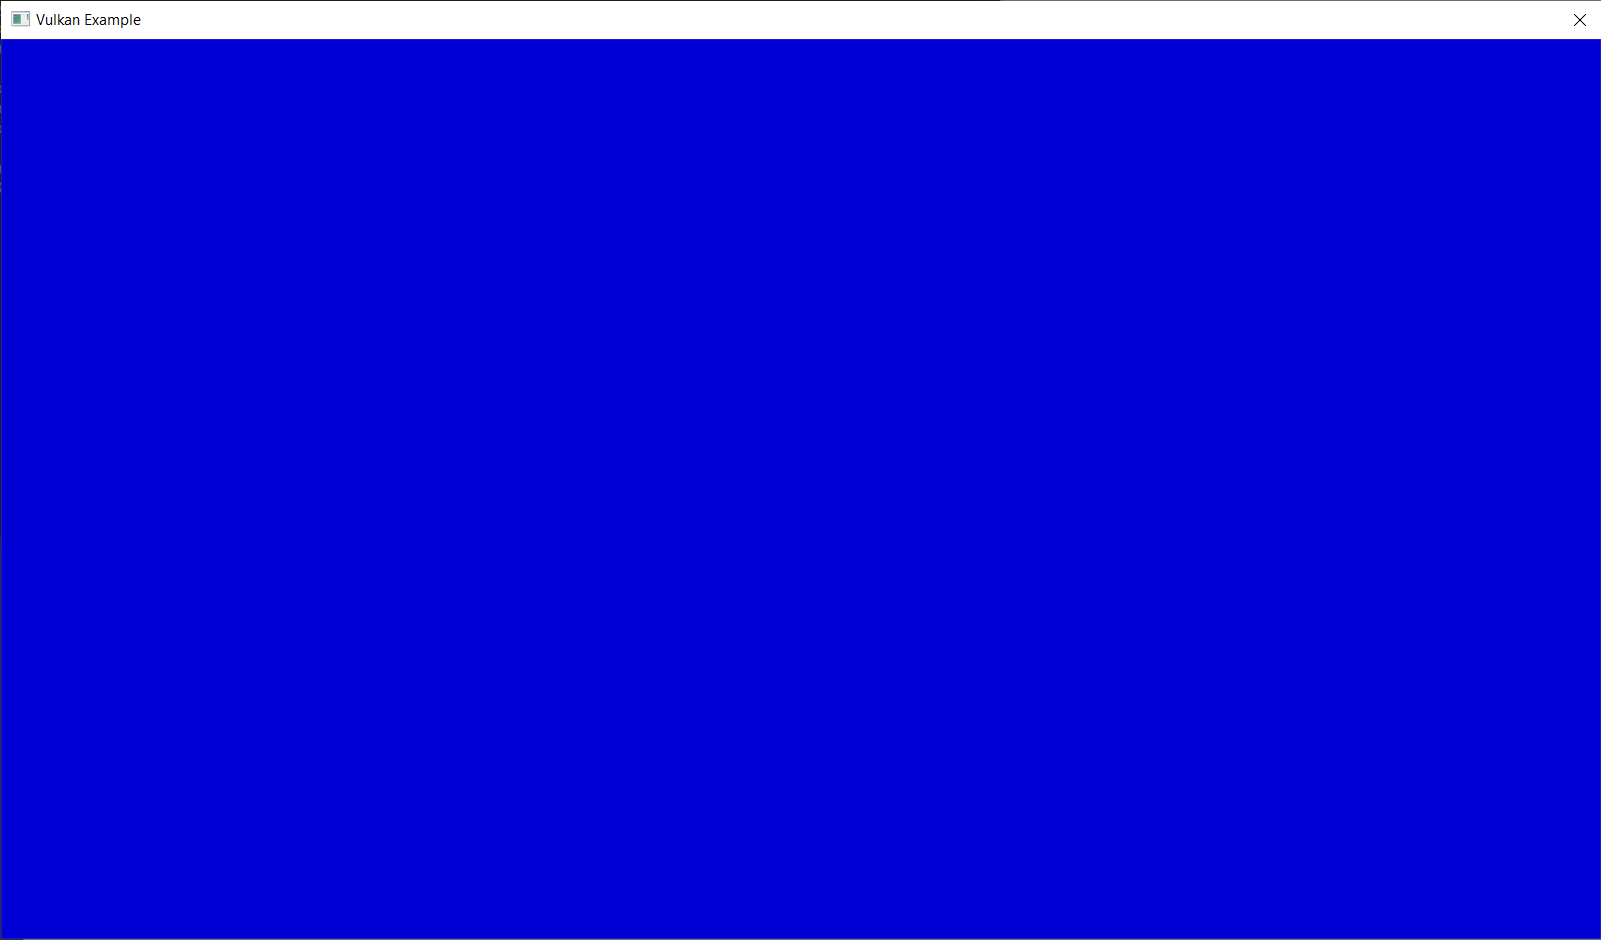
\includegraphics[scale=0.25]{images/SlidesClearWindow/ClearWindow.png}
\end{figure}
\end{frame}

\begin{frame}
\frametitle{Renderizzare Un Colore}

\begin{itemize}
\item Creiamo un render pass
\item Un render pass descrive gli attachment che vengono utilizzati durante il rendering
\item Un render pass raggruppa i comandi grafici in uno o più subpass in base a come e quali attachment utilizzano
\item Creiamo un framebuffer
\item Un reamebuffer è l'insieme di attachment utilizzati da un'istanza di un render pass
\item Creiamo un command buffer
\item Scriviamo comandi sul command buffer
\item Inviamo il command buffer alla GPU
\item Presentiamo un'immagine della swapchain sulla presentation surface
\end{itemize}
\end{frame}
